\documentclass[a4paper]{article}
\usepackage[latin1]{inputenc}
\usepackage[T1]{fontenc}
\usepackage[francais]{babel}
\usepackage{entete}
\usepackage{noitemsep}
\usepackage{euscript} 
\usepackage{amsmath,amssymb,amsfonts,amsthm}
\usepackage{graphicx,graphics,epsfig,subfigure,color}
\usepackage{url}
%\usepackage{algorithm2e}
\usepackage{multicol}
\usepackage{a4wide}
\usepackage{latexsym}
\usepackage{verbatim}
\setlength{\textheight}{23.6cm}
\setlength{\topmargin}{-1cm}
\setlength{\textwidth}{165mm}
\setlength{\oddsidemargin}{1.5mm}

\usepackage{pdfpages}
%\renewcommand{\baselinestretch}{0.85}

\pagenumbering{gobble}  %% remove page number

%\input{macroAlgo}
%\dontprintsemicolon

\setlength{\parindent}{0pt}  %%suppression indentation

\newif\ifcorrection
\correctiontrue   %% With correction
\correctionfalse   %% Reviewer's version


\begin{document}
\selectlanguage{francais}
\author{D. Fourer, L. Lagon}
\newcommand{\universityname}{IUT d'\'Evry Val d'Essonne}
\newcommand{\deptname}{D\'epartement TC (S3)}
\newcommand{\years}{2023-2024}

%------------------- TITRE -----------------------------------------
\date{Septembre 2021} 
\TDHead{\universityname}{\deptname}{R3.07, \years}{\large DS1: Probabilit\'es et statistiques appliqu\'ees}
%\TDHead{DUT TC}{}{\large TIC3: Fonctions avanc\'ees d'un tableur}
%-------------------------------------------------------------------
\vspace{-0.5cm}
\begin{center}
 \textbf{Dur\'ee 1h30, documents et objets connect\'es interdits. }\\
 \textit{Chaque r\'eponse devra \^etre r\'edig\'ee en fran\c{c}ais, \^etre intelligible et parfaitement justifi\'ee.}\\% (1 point de pr\'esentation)}
\end{center}

% \vspace{-0.3cm}
% \underline{Rappels:} 
% \begin{itemize}
% % \item Loi binomiale $X \sim \beta(n,p)$: $P(X=x) = C_n^x p^x(1-p)^{n-x}$
% % \item Loi de Poisson $X \sim \mathcal{P}(\lambda)$: $P(X=x)=\frac{\ee^{-\lambda}\lambda^x}{x!} \quad ,\forall \lambda > 0$
% % \item Esp\'erance: $E[X] = \sum_x x~P(X=x)$
% % \item Variance: $V[X] = E[(X-E[X])^2] = E[X^2] - E[X]^2$
% \end{itemize}

\vspace{-0.5cm}
%\section{Compr\'ehension du cours (5 points)}
%\vspace{-0.3cm}
%R\'epondez \`a chaque question pr\'ecis\'ement en exposant clairement vos id\'ees en une phrase maximum.

%\vspace{-0.5cm}
%% 1 point

%\exost Questions de cours (2 points)
%\begin{enumerate} %% 1,5
%\item (1 point) Quelle information apporte une mesure de probabilit\'e? Sur quel intervalle sont born\'ees ses valeurs?%1
% \ifcorrection
 %\textcolor{red}{~\\Une probabilit\'e donne une indication sur l'intervalle $[0;1]$ la possibilit\'e qu'un \'ev\'enement al\'eatoire
 %se r\'ealise. Plus cette probabilit\'e est importante, plus l'\'ev\'enement al\'eatoire est susceptible de se r\'ealiser.}
 %\fi
 %\item (1 points) Quelles propri\'et\'es v\'erifient 2 \'ev\'enements al\'eatoires $A$ et $B$ qui sont ind\'ependants entre eux?
 %%(c-\`a-d. dont la r\'ealisation de l'un ne d\'epend pas de l'autre) %2
 % \ifcorrection
 %\textcolor{red}{2 \'ev\'enements $A$ et $B$ ind\'ependants v\'erifient $P(A|B) = \frac{P(A\cap B)}{P(B)} = \frac{P(A)P(B)}{P(B)=P(A)}$ et resp. $P(B|A)=P(B)$.}
 %\fi
%\end{enumerate}

%\section{Exercices d'application du cours (15 points)} %(4 points)
%Les exercices suivants sont ind\'ependants et peuvent \^etre trait\'es dans n'importe quel ordre.

\exost D\'enombrement et probabilit\'es (8 points):
\begin{enumerate}
%  \item (2 points) Combien de mots diff\'erents de 5 caract\`eres distincts peut-on composer avec un clavier disposant de 10 lettres distinctes?
%    \ifcorrection
%  \textcolor{red}{Il s'agit d'un tirage ordonn\'e sans remise de $k=5$ parmi $n=10$, soit $N = A_{10}^5 = \frac{10!}{5!} = 6\times 7 \times 8 \times 9 \times 10 = 30240$} % $A_{30}^7 = \frac{26!}{19!} = 20 \times 21 \times ... \times 26 = 3~315~312~000 
%  \fi
%  \item (2 points) Un jeu de hasard consiste \`a trouver la bonne combinaison de 4 chiffres compris entre 1 et 49 choisis al\'eatoirement sans remise.
%    Quelle est la probabilit\'e de gagner \`a un tel jeu?
%    \ifcorrection

 \item (2 points) Au poker, les mains comptent 5 cartes dans un jeu de 32 cartes. Combien de mains comportent la reine de Coeur ? 
    \ifcorrection
 \textcolor{red}{(tirage ordonn\'e sans remise) La reine de coeur est fixe, pour le reste, il y a $\binom_{4}{31} = \frac{31!}{27!} = 485460$ mains}
 \fi
 
 \item (2 points) Le digicode ci-dessous est plac\'e \`a l'entr\'ee d'un immeuble. Le code est compos\'e de 4 symboles. Combien y a t'il de codes possibles ?
\begin{figure}[!h]
    \centering
    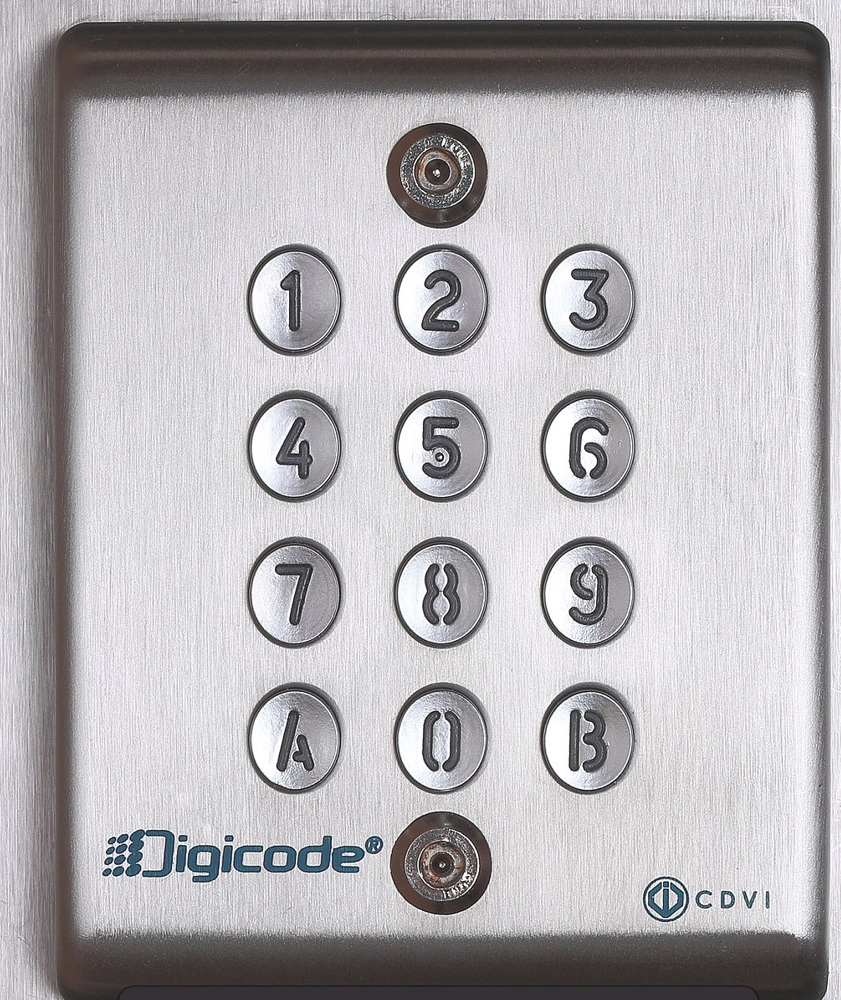
\includegraphics[width=0.2\linewidth]{digicode.jpg}
\end{figure}
   \ifcorrection
 \textcolor{red}{Il existe $12^4 = 20736$ codes possibles}
 \fi
 \item (2 points) Dans une course de F1, 20 pilotes s'affrontent. Combien y a t'il de podiums possibles ? 
    \ifcorrection
  \textcolor{red}{Il s'agit d'un tirage ordonn\'es sans remise. Il y a donc $A_{20}^3=\dfrac{20!}{17!}=6840$ podiums possibles
  \fi
  
 %\item (2 points) Un jeu de hasard consiste \`a trouver la bonne combinaison de 4 chiffres compris entre 1 et 49 choisis al\'eatoirement sans remise.
 %  Quelle est la probabilit\'e de gagner \`a un tel jeu si tous les tirages sont \'equiprobables?
 %  \ifcorrection
 %  \textcolor{red}{Il existe $N = C_{49}^4 = \frac{49!}{4!(45)!} = 211~876$ combinaisons diff\'erentes. Donc la probabilit\'e de gagner \`a ce jeu est de %$\frac{1}{N}\approx 4,71\times 10^{-6}$ }
 %  \fi
%%%%%%%%%% je suis ici
%  
%  \item Un jeu de consiste \`a trouver la bonne combinaison de 6 chiffres compris entre 1 et 49 choisis al\'eatoirement sans remise.
%   Quelle est la probabilit\'e de gagner \`a un tel jeu?
%     \ifcorrection
%  \textcolor{red}{Il existe $N = C_{49}^6 = \frac{49!}{6!(43)!} = \frac{44 \times 45 \times 46 \times 47 \times 48 \times 49}{2 \times 3 \times 4 \times 5 \times 6} = 13~983~816$ 
%  soit une probabilit\'e de $\frac{1}{N}$ pour gagner.}
%  \fi
\end{enumerate}


\exost (5 points) Une entreprise a une probabilit\'e de 1\% de signer un contrat avec chaque client
qu'elle rencontre. Elle se dote d'un logiciel d'IA qui lui permet de pr\'evoir \`a l'avance si un client va signer un contrat ou non. L'entreprise remarque que lorsqu'un client signe un contrat, l'IA avait r\'eussi \`a pr\'edire sa signature avec une fiabilit\'e de 95\%. Lorsque le client ne signe pas le contrat, l'IA avait r\'eussi \`a pr\'edir la non signature avec une fiabilit\'e de 99,5\% . \\
Ce logiciel d'IA est-il vraiment efficace ? Pour vous en assurer, vous calculerez la probabilit\'e
qu'un client signe un contrat lorsque cela a \'et\'e pr\'evu par le logiciel et vous la comparerez \`a un seuil fix\'e \`a 60\%.

 \ifcorrection
 \textcolor{red}{
 On note $S = \{\text{Un client signe un contrat}\}$ et $T=\{\text{Prediction de signature par le logiciel d'IA}\}$\\
 On a alors $P(T|S) = 0.95$, $P(T|\bar{S}) = 5\times 10{-3}$ et $P(S) = 10^{-2}$.\\
 Le th\'eor\`eme des probabilit\'e totales permet de calculer:
 $P(T) = P(T|S)P(S) + P(T|\bar{S})P(\bar{S}) = 0,95 \times 10^{-2} + 5\times 10{-3} \times (1-10^{-2}) = 1,45 \times 10^{-2}$.\\
 Le th\'eor\`eme de Bayes nous permet d'\'ecrire: 
 $P(S|T) = \frac{P(T|S)P(S)}{P(T)} = \frac{0,95 \times 10^{-2}}{1,45 \times 10^{-2}} \approx 0,6552 > 0.6$\\
 On en d\'eduit que le syst\`eme de d\'etection est bien efficace!}
 \fi
 
\end{document}

% End Of File

